\documentclass[problem]{mcs}

\begin{pcomments}
  \pcomment{from: S09.cp9r}
  \pcomment{has a pset problem associated with it}
\end{pcomments}

\pkeywords{
  counting
  bijections
  trees
}

%%%%%%%%%%%%%%%%%%%%%%%%%%%%%%%%%%%%%%%%%%%%%%%%%%%%%%%%%%%%%%%%%%%%%
% Problem starts here
%%%%%%%%%%%%%%%%%%%%%%%%%%%%%%%%%%%%%%%%%%%%%%%%%%%%%%%%%%%%%%%%%%%%%

\hyperdef{numbered}{trees}{\begin{problem}}
A \emph{numbered tree} is a tree whose vertex set is
$\set{1,2,\dots,n}$ for some $n \geq 2$.  We define the \emph{code} of
the numbered tree to be a sequence of $n-2$ integers from 1 to $n$
obtained by the following recursive process:
\begin{quotation}
If $n=2$, stop---the code is the empty sequence.  Otherwise, write down
the \emph{father} of the largest leaf\footnote{The necessarily unique node
adjacent to a leaf is called its \emph{father}.}, delete this \emph{leaf},
and continue the process on the resulting smaller tree.
\end{quotation}

For example, the codes of a couple of numbered trees are shown in 
the Figure~\ref{codetrees}.

\begin{figure}[htb]
\begin{center}
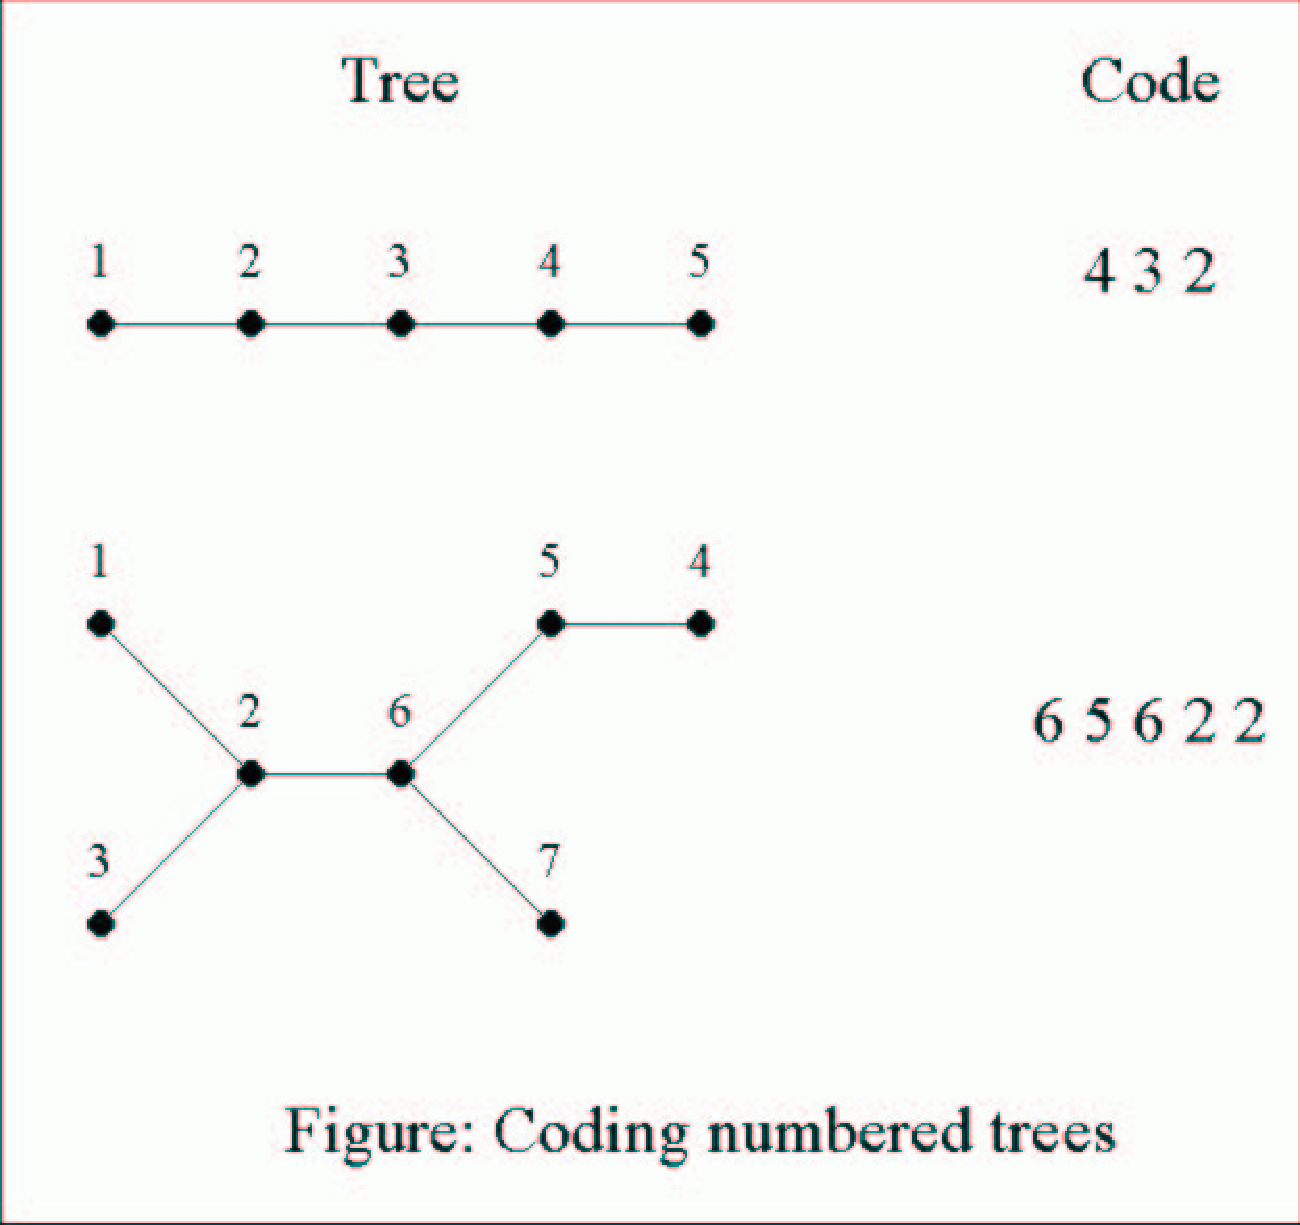
\includegraphics[width=4in]{figures/n-2}
\end{center}
\caption{}
\label{codetrees}
\end{figure}

\bparts

\ppart Describe a procedure for reconstructing a numbered tree from
its code.

\solution{
The key observation is that, given a code of length $n-2$, the numbers
between 1 and $n$ which \emph{do not appear} in the code must be leaves of
the tree.  Hence, the largest missing number is a leaf attached to the
first number of the code.  The rest of the tree can now be reconstructed
by deleting the first number in the code, henceforth ignoring the largest
leaf, and proceeding recursively on the rest of the code.  (We're using
the obvious fact that what's left after deleting a leaf from a tree is
another tree.)

More precisely, the reconstruction procedure applies to any finite tree
whose vertex set is totally ordered.  The procedure takes \emph{two}
parameters: the vertex set, $V$, and a length $\card{V}-2$ ``code''
sequence, $S$, of elements in $V$.  If $l$ is the largest element in $V$
which does not appear in $S$, and $f$ is the first element of $S$, then
the reconstructed tree is obtained by adding edge $(l,f)$ to the tree
reconstructed by calling the procedure recursively with first argument
$V-\set{l}$ and second argument equal to the code obtained by erasing the
initial $f$ from $S$.  The procedure terminates when $\card{V}=2$,
returning the edge between the two numbers in $V$.

%This paragraph is correct, but would benefit from a rewrite:

To justify the key observation, note that any vertex that gets deleted by
the process and was not a leaf to begin with, must have been the father of
a previously deleted leaf, which means it would appear in the code.  So
the missing integers must have been leaves to begin with or must be one of
the two undeleted vertices left when the coding process terminates.  But
by the end of the process the two remaining vertices are leaves, and if
they weren't leaves to begin with, they must have become leaves by having
their sons deleted, which means they would not have been missing from the
code.  So the two vertices remaining at the end must also have been leaves
of the original tree.
}

\ppart How many numbered trees with $n$ vertices are there?  Justify
your answer assuming the result of the previous problem part.

\solution{There are exactly as many $n$-vertex numbered trees as the
number of possible code words, that is, the number of length $n-2$
sequences of integers between 1 and $n$.  So there are $n^{n-2}$ numbered
trees.
  
The reason is that the map from trees to codes is a bijection.  To see
this, note that the tree reconstruction procedure finds \emph{the only
possible tree} with that code.  So there can't be two trees with the same
code, i.e., the map from a tree to its code is an injection.  But since
the reconstruction procedure finds a tree for every possible codeword, the
map from trees to codes is also a surjection.}

\eparts
\end{problem} 

%%%%%%%%%%%%%%%%%%%%%%%%%%%%%%%%%%%%%%%%%%%%%%%%%%%%%%%%%%%%%%%%%%%%%
% Problem ends here
%%%%%%%%%%%%%%%%%%%%%%%%%%%%%%%%%%%%%%%%%%%%%%%%%%%%%%%%%%%%%%%%%%%%%
